





\section{DENSEWORLD: A Benchmark for Populous, Crowded, and Chaotic Global South}

We use DENSEWORLD to denote a critical but underrepresented world-modeling regime: populous, crowded, and chaotic Global South urban scenes. It is defined not only by geography, but by measurable properties: high agent count density, high agent occupancy, persistent occlusion, agent heterogeneity, and interaction pressure. This regime matters because many emerging urban environments combine high population density, mixed mobility systems, diverse infrastructure patterns, and rapid spatial change, making them scientifically important yet underrepresented in world-model benchmarks \cite{mahendra2021seven,ellis2016leveraging}. Thus, world models must handle uncertainty, density, and relational complexity that is less prominent in lower-density, lane-structured benchmarks. See Figure~\ref{fig:denseworld_scene_types} for representative DENSEWORLD scenes.

% factor figure split into two separate single-column figures (Fig 3 + Fig 4), placed further down with body text between them (below).



We characterize DENSEWORLD through four coupled properties. First, it exhibits soft spatial boundaries: road edges, drivable space, and pedestrian regions are often negotiated rather than crisply marked \cite{varma2019idd, dokania2023idd3d}. Second, it contains extreme agent heterogeneity, with pedestrians, cars, two-wheelers, carts, animals, delivery vehicles, and rickshaws coexist locally \cite{khan1999heterogeneous,asaithambi2012mixedtraffic}. Third, it has persistent occlusion from density, clutter, and near-field encounters, producing severe partial observability \cite{varma2019idd, dokania2023idd3d}; prediction must rely on \emph{memory}, \emph{object permanence}, and \emph{relational inference}, not only visible appearance. Fourth, motion is governed less by rigid rule compliance than by rapid social negotiation under mixed traffic and weak lane discipline \cite{papathanasopoulou2018weaklane,asaithambi2012mixedtraffic}.

Together, these properties make DENSEWORLD a natural stress test for world models: success requires representations that preserve layout, agent state, and interaction dynamics under uncertainty, rather than collapsing into one entangled predictive latent. As detailed below, we measure this regime through agent count density, agent occupancy, occlusion pressure, interaction pressure, and agent heterogeneity. This motivates a predictor that separates layout, entities, and interactions.

\begin{figure}[b]
    \centering
    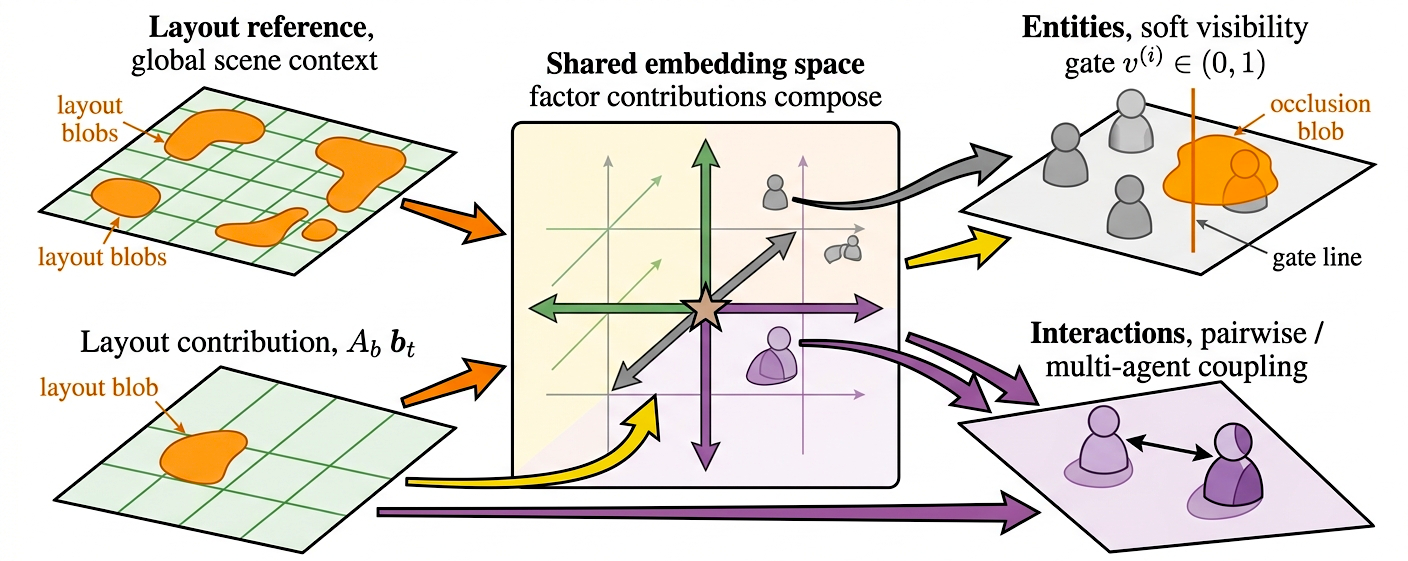
\includegraphics[width=\columnwidth]{figures/factor_visual.png}
    \caption{\textbf{\emph{Factorized predictive channels.}} Context is split into \emph{layout}, visibility-gated \emph{agent}, and sparse \emph{interaction} coordinates, then recomposed in the future JEPA embedding, limiting cross-factor leakage.}
    \label{fig:factorjepa_visual}
\end{figure}


\subsection{DENSEWORLD 1.0: the Benchmark}
\label{sec:denseworld_dataset}


We collected 714 long-form YouTube videos at 480p, totalling
276 hours of urban footage across 22 Tier-1 and Tier-2 cities in India. The data spans drive-through, walk-through, and aerial viewpoints, and long-form recordings are segmented using scene-detection and shot-boundary methods into 115,687 short videos of 4 to 10 seconds, of which 86,831 carry automatically derived layout, agent, and interaction targets. DENSEWORLD 1.0 covers commercial, residential, transit, heritage, coastal, and high-density street settings, including markets, commercial streets, transit corridors, junctions, flyovers, bazaars, ghats, beaches, and skylines. It further spans variations in the time of day, weather, crowd density, traffic mix, pedestrian--vehicle separation, road geometry, surface quality, encroachment, and lighting. Beyond standard urban actors, the dataset includes locally frequent agents and objects such as auto-rickshaws, cycle rickshaws, street vendors, and animals. Before release, all footage is processed through privacy-preserving filters, including face and license-plate blurring and removal of sensitive segments.

A defining feature of DENSEWORLD is heterogeneous mixed traffic. In many developing-country cities, multiple vehicle and actor types share the same right of way under weak lane discipline, with strong lateral and longitudinal coupling \cite{khan1999heterogeneous,papathanasopoulou2018weaklane,asaithambi2012mixedtraffic}. This is not a mild variant of standard traffic, but a qualitatively different operating regime. Prior work highlights the coexistence of cars, buses, trucks, auto-rickshaws, scooters, motorcycles, bicycles, carts, and other slow- and fast-moving agents within the same corridor \cite{khan1999heterogeneous,asaithambi2012mixedtraffic}. Here, scene structure does not decompose into \emph{static lanes}, \emph{isolated actors}, and \emph{simple pairwise relations}; spatial support is fluid, visibility is unstable, and behavior is shaped by dense local negotiation.

\begin{figure}[t]
    \centering
    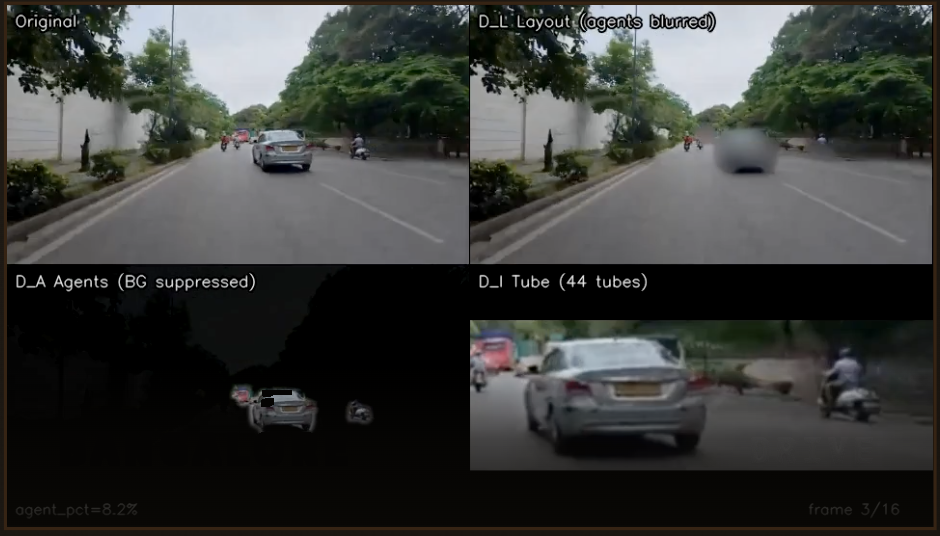
\includegraphics[width=0.95\columnwidth]{figures/segmented_scene.png}
    \caption{\textbf{\emph{DINO-based factor-target construction.}} Per clip, the pipeline derives \emph{layout} $D_L$, \emph{agent} $D_A$, and \emph{interaction} $D_I$ supervision by masking foreground/background and linking agent tubes.}
    \label{fig:dino_factor_targets}
\end{figure}









\subsection{How Dense is DENSEWORLD? Comparison with Standard Driving Benchmarks}

% Figure denseworld_vs_west_density relocated to 2_factor_jepa.tex (after the factor-view figures) per layout request; it now renders as Fig 5.

To make this regime measurable, we compare DENSEWORLD against BDD100K and nuScenes, two widely used benchmarks for autonomous-driving perception and scene understanding~\cite{yu2020bdd100k,caesar2020nuscenes}. The goal is not to claim that DENSEWORLD scenes merely look different, but to test whether they occupy a quantitatively distinct operating regime for world-model evaluation.

We measure this regime along five axes: agent count density, agent occupancy, occlusion pressure, interaction pressure, and agent heterogeneity. These metrics capture, respectively, the number of dynamic agents, the fraction of image area they occupy, the frequency of partial or heavy occlusion, the density of spatially proximate agent pairs, and the diversity of co-occurring actor categories. Together, they quantify the multi-agent load, visual congestion, visibility degradation, local interaction structure, and traffic diversity of each scene.

For an auditable comparison, all statistics are computed after mapping labels to a shared dynamic-agent taxonomy and matching comparable scene categories across datasets. 
%The full taxonomy mapping and scene-matching protocol are provided in Appendix~\ref{app:shared_taxonomy}.
DENSEWORLD has consistently higher density and occupancy across matched categories, with the largest gaps in market, commercial, and flyover/underpass scenes (quantified in the supplementary material). These results support the central premise of the benchmark: DENSEWORLD is not merely a geographic extension of existing driving data; it defines a higher-density, higher-occlusion, and higher-interaction regime for evaluating predictive world models. Full automatic-annotation details, including thresholds, annotation taxonomy, export format, and loss mapping, are provided in Appendix~C.